\documentclass[../TinyBot.tex]{subfiles}
% \graphicspath{{resources/}}
\begin{document}

\section{Wiring} \label{wiring}
If you just want to see the wiring schematic, see Figure \ref{fig:schematic-hbridge-battery}. Continue reading for an explanation of the L293D H-Bridge and of the circuit. 

\bigskip

Before starting construction on any project, it is always a good idea to wire up the circuit on a flat breadboard and Arduino; as it is far easier to build the circuit on its own before putting together all the parts. \\

\begin{warningbox}
    There are two different kinds of wires, solid core and multi core. \\

    
    Multicore wire is more common, and is better suited for soldering as the strands in two wires can mesh together and the solder  wraps around all the strands and forms a better bond between the wires. Multicore wire is annoying to use with breadboards as individual strands can be bent and not plug in correctly. This can often be fixed by "tinning" the wires, where the stripped ends of the wires are coated in a thin layer of solder to hold all the strands together.\\

    Solid core wire is made of a single thicker strand of wire, making it better for bread boarding as there are no thin strands to be pushed out of shape. However, solid core wire is terrible for soldering as good connections are hard to ensure. \\


    % Solid core wire is better for prototyping with breadboards as it is easier to plug the wire into the board. Multicore wire is better for soldering as a better connection is made between two pieces of multicore wire as the strands can mesh together, the solder also wraps around all the strands and forms a better bond between the wires. \\

    % Solid core is very useful when using breadboards where as multicore is better for soldering. 
    The club has both solid core and multi core wire, double check you have solid core on hand as this will make wiring the circuit much easier. Solid core wire is also very easy to cut to length to create neater looking circuits. \\
    
\end{warningbox}


\begin{center}
    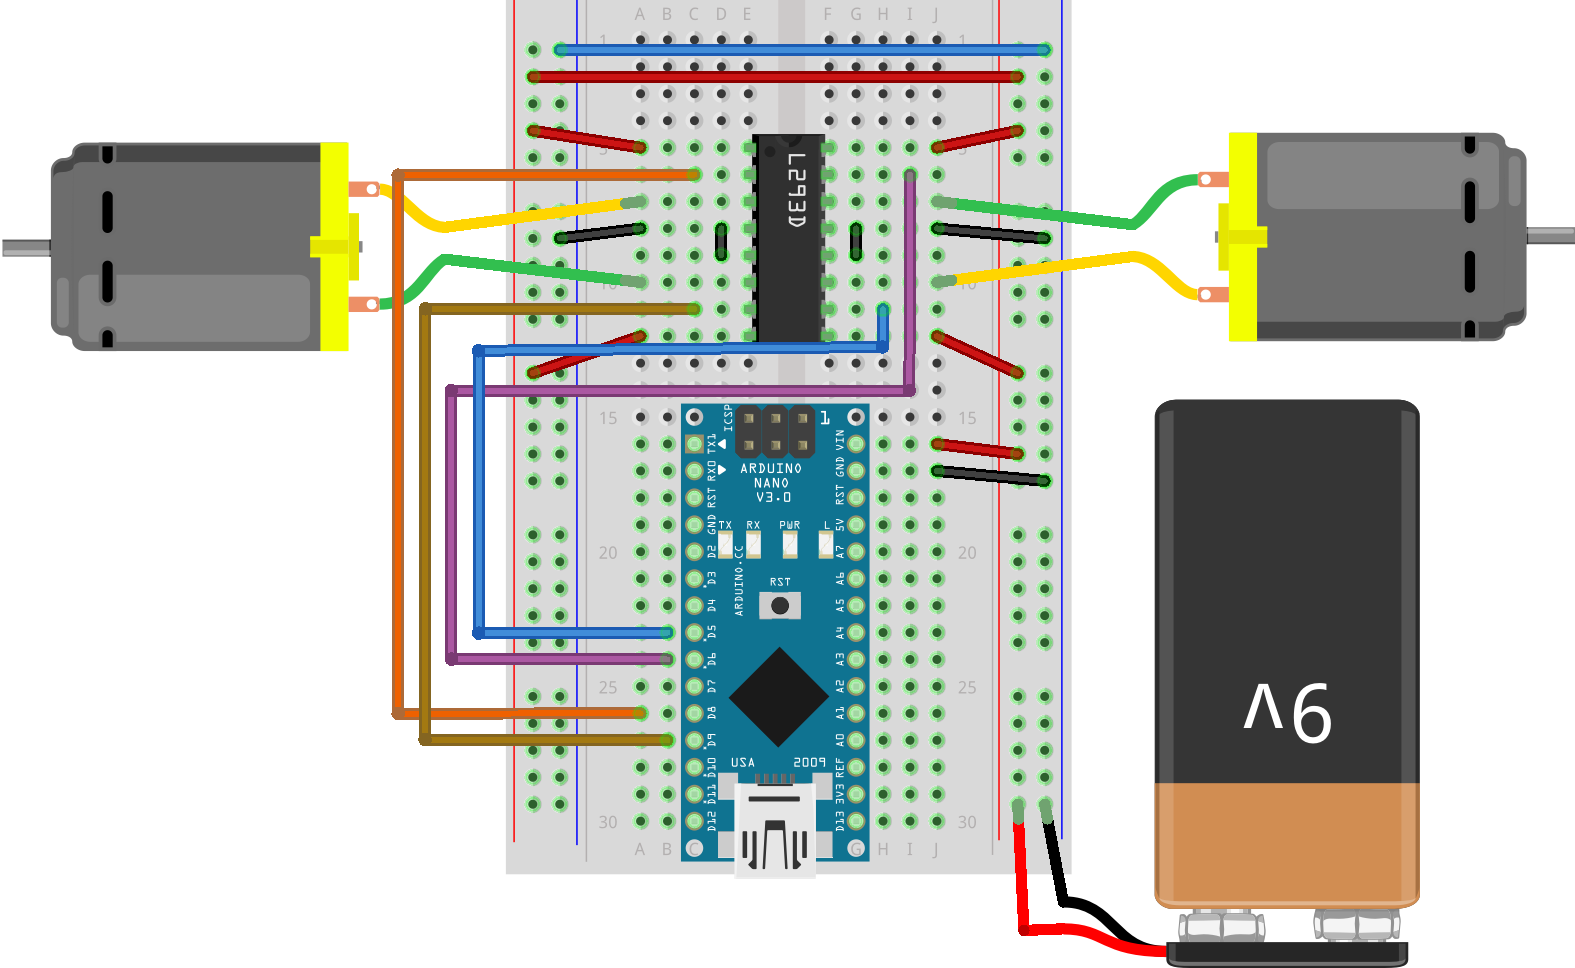
\includegraphics[width=\textwidth]{resources/H-bridge-nano_bb.png}
    \captionof{figure}{Wiring Schematic for H-Bridge}
    \label{fig:schematic-hbridge-battery}
\end{center}

Make sure to check which wire is the positive wire on the motor you have, it should be written on the back plate of the motor. Plugging the motor in backwards will not break anything, the motor will just spin backwards. 

Swapping the motor direction can be done by swapping the green and yellow wires attached to the motor. 
% It is mainly important to ensure that the motors spin in the same direction. 
\\

If you don't have a battery, the circuit is mostly the same; though with some differences with how power is supplied to the circuit. Instead of powering the Arduino and circuit with the 9V battery you power the Arduino through USB and the circuit from the 5V output pin. See below for a wiring diagram without the battery.


\begin{center}
    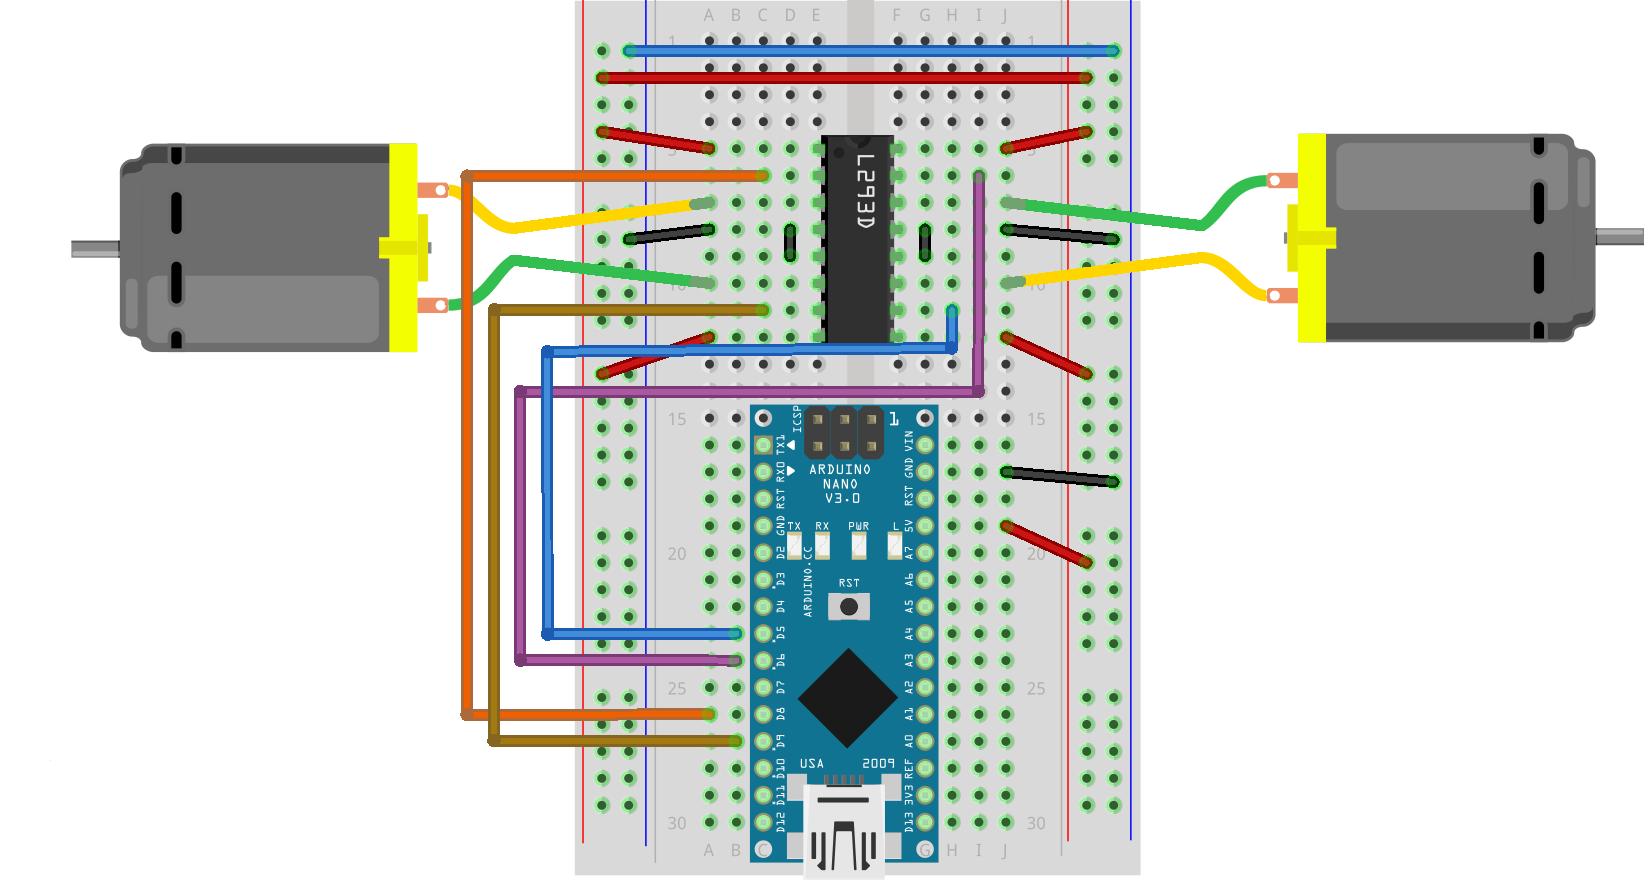
\includegraphics[width=\textwidth]{resources/H-bridge-nano-without-battery_bb.png}
    \captionof{figure}{Wiring Schematic for H-Bridge}
    \label{fig:schematic-hbridge-nobattery}
\end{center}


The circuit in real life will look something like in Figure \ref{fig:circuit-wired-irl}

\begin{center}
    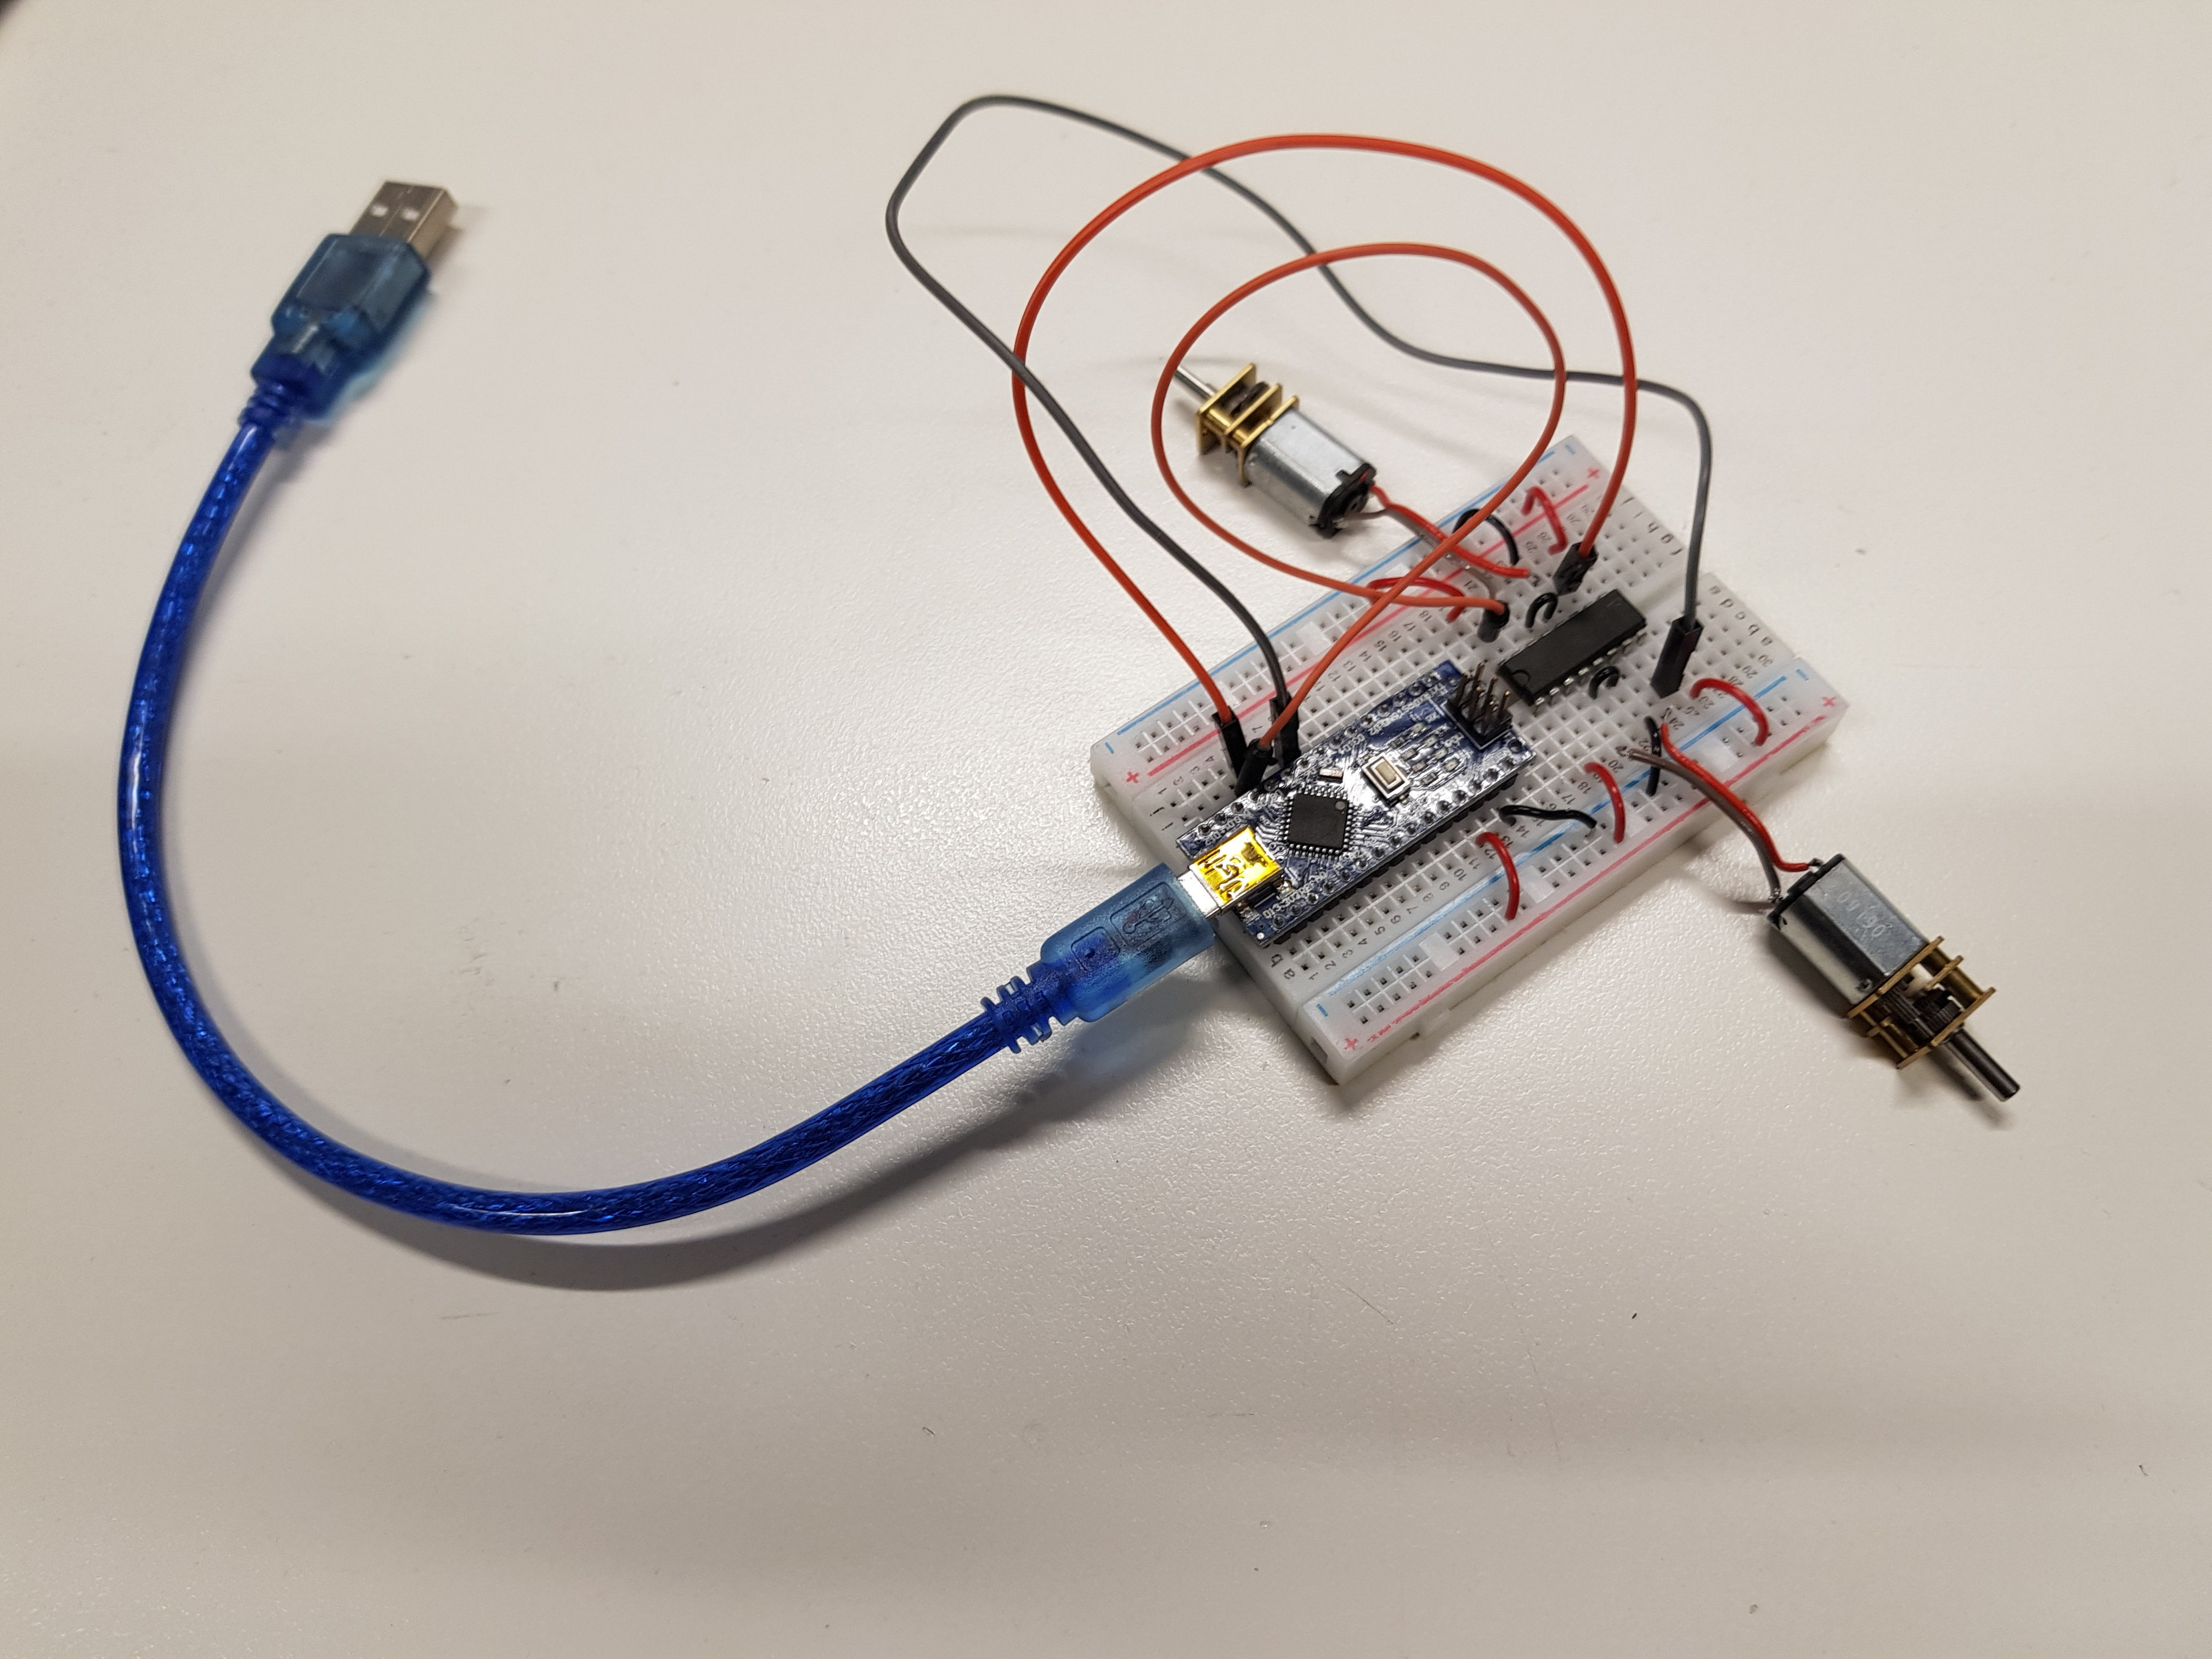
\includegraphics[width=0.7\textwidth]{circuit_wired.jpg}
    \captionof{figure}{Wired Circuit}
    \label{fig:circuit-wired-irl}
\end{center}


\end{document}